% !TEX TS-program = pdflatex
% academicthesis-polimi-guide.tex
% User and developer guide of the academicthesis class for Politecnico di
% Milano. Compile from this folder with pdfLaTeX, twice:
%   pdflatex academicthesis-polimi-guide.tex
% Standalone: it does not need the academicthesis class itself.
\documentclass[11pt,a4paper,oneside]{report}
\newcommand{\doctitleshort}{academicthesis --- Politecnico di Milano guide}
% common/docstyle.tex
% Shared preamble of the academicthesis guides (one guide per university).
% \input it right after \documentclass{report}. A guide sets its accent
% colour afterwards with \colorlet{docaccent}{...}. The guides are
% standalone: they do not need the academicthesis class itself.
\usepackage[T1]{fontenc}
\usepackage[utf8]{inputenc}
\usepackage{lmodern}
\usepackage[english]{babel}
\usepackage[a4paper, margin=2.6cm, headheight=14pt]{geometry}
\usepackage{microtype}
\usepackage{xcolor}
\usepackage{graphicx}
\usepackage{array}
\usepackage{tabularx}
\usepackage{booktabs}
\usepackage{longtable}
\usepackage{listings}
\usepackage{enumitem}
\usepackage{titlesec}
\usepackage{titletoc}
\usepackage{fancyhdr}
\usepackage{tcolorbox}
\tcbuselibrary{skins, breakable}
\usepackage{tikz}
\usetikzlibrary{positioning, arrows.meta}
\usepackage{url}
\usepackage[colorlinks=true, linkcolor=docaccent, urlcolor=docaccent,
            citecolor=docaccent]{hyperref}

% ---- Colours (docaccent is set again by each guide) -------------------
\definecolor{docaccent}{RGB}{31,73,125}
\definecolor{luissblue}{RGB}{21,57,108}      % BlueLuiss, as in the package
\definecolor{bluepoli}{cmyk}{0.4,0.1,0,0.4}  % bluepoli, as in the package
\definecolor{bocconiblue}{RGB}{0,46,93}
\definecolor{docgrey}{gray}{0.45}

% ---- Page and paragraphs ----------------------------------------------
\setlength{\parindent}{0pt}
\setlength{\parskip}{0.55\baselineskip}
\setlength{\emergencystretch}{3em}
\sloppy
\setlist{nosep, topsep=3pt, leftmargin=1.5em}
\renewcommand{\arraystretch}{1.25}
\usepackage{etoolbox}
\AtBeginEnvironment{tabularx}{\small}
\AtBeginEnvironment{longtable}{\small}

% Parts: a full page with a large number and a short description
% \guidepart{<title>}{<one-paragraph introduction>}
\newcommand{\currentpartintro}{}
\titleformat{\part}[display]{\centering\color{docaccent}}
  {\Large\scshape Part \thepart}{10pt}{\Huge\bfseries}
  [\vspace{1.2cm}\begin{minipage}{0.72\linewidth}\centering
   \normalfont\normalsize\color{black}\currentpartintro\end{minipage}]
\newcommand{\guidepart}[2]{\renewcommand{\currentpartintro}{#2}\part{#1}}

\titleformat{\chapter}[display]{\color{docaccent}\normalfont}
  {\large\scshape Chapter \thechapter}{4pt}{\Huge\bfseries}
  [\vspace{2pt}{\color{docaccent}\titlerule[0.8pt]}]
\titlespacing*{\chapter}{0pt}{0pt}{22pt}
\titleformat{\section}{\color{docaccent}\normalfont\Large\bfseries}{\thesection}{0.8em}{}
\titleformat{\subsection}{\color{docaccent}\normalfont\large\bfseries}{\thesubsection}{0.8em}{}
\titleformat{\subsubsection}{\normalfont\normalsize\bfseries}{\thesubsubsection}{0.8em}{}
\titlespacing*{\section}{0pt}{2.4ex plus 1ex}{1ex}
\setcounter{tocdepth}{1}

\pagestyle{fancy}
\fancyhf{}
\fancyhead[L]{\small\color{docgrey}\doctitleshort}
\fancyhead[R]{\small\color{docgrey}\nouppercase{\leftmark}}
\fancyfoot[C]{\small\thepage}
\renewcommand{\headrulewidth}{0.3pt}
\renewcommand{\chaptermark}[1]{\markboth{\thechapter\quad #1}{}}
\fancypagestyle{plain}{\fancyhf{}\renewcommand{\headrulewidth}{0pt}\fancyfoot[C]{\small\thepage}}
\providecommand{\doctitleshort}{academicthesis}

% ---- Names in running text and tables ---------------------------------
\newcommand{\cs}[1]{\texttt{\textbackslash#1}}   % a command
\newcommand{\opt}[1]{\texttt{#1}}                 % an option / key / value
\newcommand{\env}[1]{\texttt{#1}}                 % an environment
\newcommand{\pkg}[1]{\textsf{#1}}                 % a package or class
\DeclareUrlCommand{\file}{\urlstyle{tt}}          % a file name (breaks at - . /)
\renewcommand{\UrlBreaks}{\do\-\do\.\do\/\do\_}
\newcolumntype{Y}{>{\raggedright\arraybackslash}X}
\newcolumntype{L}[1]{>{\raggedright\arraybackslash}p{#1}}
\newcommand{\req}{\textbf{required}}
\newcommand{\optional}{optional}
\newcommand{\na}{\textcolor{docgrey}{---}}

% ---- Code listings -----------------------------------------------------
\lstset{
  basicstyle=\ttfamily\small,
  keywordstyle=\color{docaccent}\bfseries,
  commentstyle=\color{docgrey}\itshape,
  language=[LaTeX]TeX,
  morekeywords={thesissetup, frontpage, luissthesissetup, polimithesissetup,
    bocconithesissetup, major, dedication, frontmatter, mainmatter,
    backmatter, addbibresource, printbibliography, blankpage,
    DeclareThesisBaseClass, DeclareThesisFormats, DeclareThesisSecondPage,
    DeclareThesisOtherLanguages, DeclareThesisClassOption,
    DeclareThesisCoreRequirements, DeclareThesisFrontPage,
    DeclareThesisRequirement, DeclareThesisBibDefaults, ProvideThesisString,
    thesismeta, thesisstring, IfThesisMetaEmptyTF, IfThesisListEmptyTF,
    IfThesisDegreeTF, academicthesislist, AddToHook, ExplSyntaxOn,
    ExplSyntaxOff, ProvidesExplPackage, ProvidesFile, RequirePackage},
  frame=single, rulecolor=\color{docaccent!35},
  backgroundcolor=\color{docaccent!4},
  columns=fullflexible, keepspaces=true, upquote=true,
  breaklines=true, breakatwhitespace=true,
  xleftmargin=4pt, xrightmargin=4pt, aboveskip=8pt, belowskip=8pt,
  literate={à}{{\`a}}1 {è}{{\`e}}1 {é}{{\'e}}1 {ò}{{\`o}}1,
}
\lstdefinestyle{shell}{language={}, keywordstyle={}, commentstyle={}}

% ---- Boxes ---------------------------------------------------------------
% \begin{notebox}[<colour>]{Title} ... \end{notebox}
\newtcolorbox{notebox}[2][docaccent]{enhanced, breakable,
  colback=#1!5, colframe=#1!70, boxrule=0.6pt, arc=2pt,
  left=8pt, right=8pt, top=6pt, bottom=6pt,
  fonttitle=\bfseries\small, coltitle=white, title={#2}}

% A framed page preview: \preview[<width>]{<file>}{<caption>}
\newcommand{\preview}[3][0.42\textwidth]{%
  \begin{minipage}[t]{#1}\centering
    {\setlength{\fboxsep}{0pt}\setlength{\fboxrule}{0.5pt}%
     \fcolorbox{docgrey!50}{white}{\includegraphics[width=\dimexpr\linewidth-1pt\relax]{#2}}}\par
    \vspace{4pt}{\small #3}
  \end{minipage}}

% ---- Title page: \guidetitlepage{<subtitle>}{<figures>} ----------------
\newcommand{\guidetitlepage}[2]{%
  \hypersetup{pageanchor=false}%
  \begin{titlepage}
    \centering
    \vspace*{0.6cm}
    \includegraphics[width=0.62\linewidth, trim=150 125 142 114, clip]{academicthesis-logo}\par
    \vspace{18pt}
    {\color{docaccent}\rule{0.8\linewidth}{1pt}}\par\vspace{12pt}
    {\LARGE\color{docaccent} #1\par}
    \vspace{6pt}
    {\Large User and developer guide\par}
    \vspace{12pt}
    {\color{docaccent}\rule{0.8\linewidth}{1pt}}\par
    \vspace{1.2cm}
    #2\par
    \vfill
    {\large Luca Salvatore\par}
    {\color{docgrey} academicthesis v0.2.0 \quad\textbullet\quad October 2026\par}
  \end{titlepage}%
  \hypersetup{pageanchor=true}}

\graphicspath{{figures/}{../assets/logo/}}

\colorlet{docaccent}{bluepoli!80!black}

\newcommand{\uniname}{Politecnico di Milano}
\newcommand{\unishort}{PoliMi}
\newcommand{\uniid}{polimi}
\newcommand{\uniotherlangnote}{English and Italian are always loaded for
  PoliMi, so an Italian abstract needs nothing more; for a third language,
  list it in the \opt{other-languages} class option.}
\newcommand{\unibibdefault}{PoliMi sets none, so the numeric style applies}

\hypersetup{pdftitle={academicthesis: Politecnico di Milano user and developer guide},
            pdfauthor={Luca Salvatore}}

\begin{document}

\guidetitlepage{Politecnico di Milano}{%
  \preview[0.21\textwidth]{polimi-classical-cover}{\opt{classical}}\hspace{0.4cm}%
  \preview[0.21\textwidth]{polimi-article-cover}{\opt{article}}\hspace{0.4cm}%
  \preview[0.21\textwidth]{polimi-summary-cover}{\opt{summary}}\hspace{0.4cm}%
  \preview[0.17\textwidth]{polimi-phd-cover}{\opt{phd}}}

{\setlength{\parskip}{0pt}\tableofcontents}

% ######################################################################
\guidepart{User guide}{For students writing a thesis, an Executive
Summary or a doctoral dissertation at Politecnico di Milano: what the
class does, how to set it up, every option and command available, and
complete examples.}

% ======================================================================
\chapter{What this package does}

Politecnico di Milano provides \LaTeX{} templates for its theses. Using a
template means copying a folder, editing its configuration by hand and
keeping track of which file prints what. \pkg{academicthesis} turns those
layouts into a class: you choose the format with one option, give the data
of the thesis once, and the class produces the cover, the headings and the
page layout of that format.

\begin{lstlisting}
\documentclass[university=polimi, master, format=classical]{academicthesis}
\end{lstlisting}

\begin{notebox}{The PoliMi layouts are Politecnico di Milano's design}
The layouts produced by this package are \textbf{not original work of
academicthesis}. They reproduce the official \LaTeX{} templates provided by
Politecnico di Milano:
\begin{itemize}
  \item the thesis templates of the School of Industrial and Information
    Engineering (Scuola di Ingegneria Industriale e dell'Informazione,
    ``Scuola 3I''), revision of October 2021: \emph{Thesis classical
    format}, \emph{Thesis article format} and \emph{Executive Summary},
    the models of the \opt{classical}, \opt{article} and \opt{summary}
    formats;
  \item the PoliMi doctoral dissertation template (\file{phdthesis.sty},
    \file{phdtitle.sty}, by J.~Stevens and L.~Fossati), the model of the
    \opt{phd} format.
\end{itemize}
The page designs, the colour \opt{bluepoli}, the cover arrangements, the
heading styles, the ``raggiera'' background and the Politecnico logos and
seal belong to Politecnico di Milano and to the authors of those
templates. This package re-implements them on the shared
\pkg{academicthesis} core, so that they are selected with a class option
and share its data handling, checks and multilingual blocks.
\end{notebox}

\section{The four formats}

\begin{center}
  \preview[0.22\textwidth]{polimi-classical-cover}{\opt{classical}}\hfill
  \preview[0.22\textwidth]{polimi-article-cover}{\opt{article}}\hfill
  \preview[0.22\textwidth]{polimi-summary-cover}{\opt{summary}}\hfill
  \preview[0.18\textwidth]{polimi-phd-cover}{\opt{phd}}
\end{center}

\begin{tabularx}{\textwidth}{@{}l Y l l@{}}
\toprule
\textbf{Format} & \textbf{What it is} & \textbf{Degrees} & \textbf{Built on} \\
\midrule
\opt{classical} & The full thesis as a book: cover page, abstracts, chapters. Default for bachelor and master. & bachelor, master & \pkg{book}, 12pt, two-sided, A4 \\
\opt{article} & The thesis as a paper: a header block with the abstract on page~1, then sections. & bachelor, master & \pkg{article}, 11pt, A4 \\
\opt{summary} & The Executive Summary, in two columns under a blue page header. & bachelor, master & \pkg{article}, 11pt, 2 columns, A4 \\
\opt{phd} & The doctoral dissertation. Default for the \opt{phd} degree. & PhD & \pkg{book}, 10pt, 17$\times$24\,cm \\
\bottomrule
\end{tabularx}

\section{What you get}

\begin{itemize}
  \item \textbf{The right base class, page size and layout} for the
    chosen format, chosen for you.
  \item \textbf{The cover or first-page block} of the format, filled from
    your data.
  \item \textbf{PoliMi headings, colours and captions}: blue chapter and
    section titles, blue caption labels, theorem and proposition
    environments in the PoliMi style.
  \item \textbf{Labels in PoliMi's wording} (``Advisor'', ``Student ID'',
    ``Master's Thesis in'') in English or Italian, following the language
    of the thesis.
  \item \textbf{An English and an Italian abstract}, with the correct
    headings and hyphenation, without extra options.
  \item \textbf{Checks}: if a field the format needs is missing,
    compilation stops with a message naming it.
\end{itemize}

\section{How it is organised}

The class has a core shared by every university and one package per
university. With \opt{university=polimi} the core loads the PoliMi package
by itself, and the PoliMi package loads the code of the chosen format.
Part~\ref{part:dev} of this guide explains the code.

% ======================================================================
% common/user-install.tex
% Shared chapter of the user part: installing and compiling.
% Uses \uniname, \unishort, \uniid, set by the guide.
\chapter{Installing and compiling}
\label{ch:install}

\section{Requirements}

\begin{itemize}
  \item A recent \TeX{} distribution: \TeX{}~Live or Mac\TeX{} 2023 or
    later, or an up-to-date MiK\TeX. The class is written in \LaTeX3 and
    needs a modern \LaTeX{} kernel.
  \item \textbf{pdf\LaTeX} is the reference engine, used by all the
    examples in this guide. Xe\LaTeX{} and Lua\LaTeX{} are also accepted
    (the class then loads \pkg{fontspec}).
  \item For the bibliography, \pkg{biblatex} and \pkg{biber}, both part of
    every full \TeX{} distribution. Without them the class falls back to
    \pkg{natbib} and Bib\TeX{} (Section~\ref{sec:bib}).
\end{itemize}

\section{The files you need}

\pkg{academicthesis} is a collection of small packages that load one
another \emph{by name}. For a \unishort{} thesis you need only these:

\begin{tabularx}{\textwidth}{@{}l Y@{}}
\toprule
\textbf{Files} & \textbf{Role} \\
\midrule
\file{core/academicthesis.cls}, \file{core/academicthesis-kernel.sty} & The core class, shared by every university. \\
\file{languages/academicthesis-<language>.ldf} & The words printed on the pages, one file per language (English, Italian, French). \\
\texttt{universities/\uniid/*} & The \unishort{} package: its layout, labels and logos. \\
\bottomrule
\end{tabularx}

The other folders of \file{universities/} belong to other universities and
can be left out.

\section{Three ways to set it up}

\begin{enumerate}
  \item \textbf{Inside the repository.} Copy the \unishort{} showcase in
    \file{showcases/} and keep its first line,
    \begin{lstlisting}
\input{academicthesis-repo-paths}
    \end{lstlisting}
    which tells \LaTeX{} where the package folders are. Then compile with
    any editor, or from a terminal with \texttt{latexmk}.
  \item \textbf{Next to your thesis.} Copy the files listed above into the
    folder of your thesis (without sub-folders) and delete the
    \verb|\input{academicthesis-repo-paths}| line. This is also how to
    use the class on Overleaf: upload the files to the project.
  \item \textbf{Installed in your personal \TeX{} tree}, for example
    \file{~/Library/texmf/tex/latex/academicthesis/} on macOS or
    \file{~/texmf/tex/latex/academicthesis/} on Linux. Every document on the
    computer can then use the class, with no extra line.
\end{enumerate}

\begin{notebox}{Editors}
Texifier/Texpad, TeXShop, TeXstudio, VS Code (LaTeX Workshop) and Overleaf
all work. In Texifier/Texpad, set the typesetter to \emph{TeX Live
(pdfLaTeX)}: its built-in engine is too old for this class.
\end{notebox}

\section{Compiling}

Run pdf\LaTeX{} twice (for the table of contents and cross-references),
with \pkg{biber} between the two runs when the thesis has a bibliography.
\texttt{latexmk} does all of this by itself:

\begin{lstlisting}[style=shell]
latexmk -pdf my-thesis.tex
\end{lstlisting}


% ======================================================================
\chapter{Writing your thesis}
\label{ch:writing}

\section{The shape of a thesis file}

\begin{lstlisting}
\documentclass[university=polimi, master, format=classical,
               language=english]{academicthesis}

\usepackage{amssymb, bm}         % your own packages, if any
\usepackage{hyperref}

\thesissetup{                    % the data printed on the cover
  title         = {Title},
  candidate     = {Name Surname},
  idnumber      = {000000},
  degree        = {Mathematical Engineering - Ingegneria Matematica},
  supervisor    = {Prof. Name Surname},
  cosupervisors = {Name Surname, Name Surname},
  academicyear  = {2025-26},
}
\addbibresource{references.bib}

\begin{document}
\frontpage                       % the cover (classical, phd) or page-1 block

\frontmatter
\begin{abstractthesis}[keywords = {first, second}]
  English abstract.
\end{abstractthesis}
\begin{abstractthesis}[language = italian, keywords = {primo, secondo}]
  Abstract in lingua italiana.
\end{abstractthesis}
\tableofcontents

\mainmatter
\chapter{Introduction}
...
\printbibliography
\end{document}
\end{lstlisting}

\section{Class options}

\begin{tabularx}{\textwidth}{@{}L{3.1cm} L{3.6cm} Y@{}}
\toprule
\textbf{Option} & \textbf{Values} & \textbf{Meaning} \\
\midrule
\opt{university} & \opt{polimi} & Selects the PoliMi package. Required. \\
degree & \opt{bachelor}, \opt{master}, \opt{phd} & Written on its own. Bachelor and master print ``Bachelor's / Master's Thesis in'' (Italian: ``Tesi di Laurea Triennale / Magistrale in''). Default: \opt{bachelor}. \\
\opt{format} & \opt{classical}, \opt{article}, \opt{summary}, \opt{phd} & The layout. Default: \opt{classical}, or \opt{phd} with the \opt{phd} degree. \opt{phd} requires that degree. \\
\opt{language} & \opt{english}, \opt{italian} & Language of every label, and hyphenation. Default: \opt{english}. \\
\opt{other-languages} & e.g.\ \opt{\{french\}} & A third language used by single blocks. \\
\opt{secondpage} & & Adds the core's examination and copyright page, which PoliMi does not use (off by default). \\
\opt{biblatex-options} & e.g.\ \opt{\{style=numeric-comp\}} & Options for \pkg{biblatex} (Section~\ref{sec:bib}). \\
anything else & \opt{11pt}, \opt{oneside}, \dots & Passed to the base class; your choice wins over the format's default. \\
\bottomrule
\end{tabularx}

\section{The data of your thesis}
\label{sec:data}

All the data is given with \cs{thesissetup} in the preamble. Write academic
titles (``Prof.'') yourself.

\subsection{Bachelor's and master's (classical, article, summary)}

\begin{longtable}{@{}L{3.0cm} L{5.4cm} c c c@{}}
\toprule
\textbf{Key} & \textbf{Printed as (English / Italian)} & \textbf{classical} & \textbf{article} & \textbf{summary} \\
\midrule
\endhead
\opt{title} & Title, in blue & \req & \req & \req \\
\opt{subtitle} & Under the title & \optional & \optional & \optional \\
\opt{candidate} & Author / Candidato & \req & \req & \req \\
\opt{idnumber} & Student ID / Matricola & \req & \req & \na \\
\opt{degree} & After ``Master's Thesis in'' & \req & \req & \req \\
\opt{supervisor(s)} & Advisor(s) / Relatore, Relatori & \req & \req & \req \\
\opt{cosupervisor(s)} & Co-advisor(s) / Correlatore, Correlatori & \optional & \optional & \optional \\
\opt{academicyear} & Academic Year / Anno Accademico & \req & \req & \req \\
\opt{abstract} & English abstract on page~1 & \na & \req & \na \\
\opt{keywords} & Its keywords, in a blue box & \na & \optional & \na \\
\opt{gender} & Candidato / Candidata (Italian) & \optional & \optional & \optional \\
\bottomrule
\end{longtable}

\subsection{Doctoral dissertation (phd)}

\begin{longtable}{@{}L{3.0cm} L{9.0cm} c@{}}
\toprule
\textbf{Key} & \textbf{Printed as (English / Italian)} & \textbf{Required} \\
\midrule
\endhead
\opt{title}, \opt{subtitle} & Title; subtitle when given & title \\
\opt{candidate} & Under ``Doctoral Dissertation of'' / ``Tesi di Dottorato di'' & \req \\
\opt{department} & In full, as printed: ``Department of Electronics, Information and Bioengineering'' & \req \\
\opt{phdtitle} & In full, as printed: ``Doctoral Program in Information Technology'' & \req \\
\opt{supervisor(s)} & Supervisor(s) / Relatore, Relatori & \req \\
\opt{tutor(s)} & Tutor(s) / Tutor & \optional \\
\opt{coordinator} & The Chair of the Doctoral Program / Il Coordinatore del Dottorato & \optional \\
\opt{academicyear}, \opt{cycle} & Bottom line: ``2025--2026 -- Cycle XXXVIII'' & \req \\
\bottomrule
\end{longtable}

\begin{notebox}{One person or several}
\opt{supervisor} takes one name and keeps any comma in it;
\opt{supervisors} takes several, separated by commas, and the label
becomes ``Advisors''. The same holds for \opt{cosupervisor(s)} and
\opt{tutor(s)}. \cs{thesissetup} can be used several times; a later value
replaces an earlier one.
\end{notebox}

\section{PoliMi options: \texorpdfstring{\cs{polimithesissetup}}{\\polimithesissetup}}

\begin{tabularx}{\textwidth}{@{}l l Y@{}}
\toprule
\textbf{Key} & \textbf{Default} & \textbf{Effect} \\
\midrule
\opt{logo-file} & \opt{logopolimi3i} & Logo on the cover or first page, file name without extension. The \opt{phd} format uses the round seal, \opt{logopolimiseal}. \\
\opt{watermark} & \opt{true} & The ``raggiera'' in the background of the cover, of page~1 and of blank pages; \opt{false} removes it. Not used by \opt{phd}. \\
\opt{paper} & \opt{17x24} & \opt{phd} only: \opt{17x24} (as in the template) or \opt{a4}. \\
\bottomrule
\end{tabularx}

\begin{lstlisting}
\polimithesissetup{watermark = false}
\end{lstlisting}

% ======================================================================
\chapter{The formats in detail}

\section{classical}

\begin{itemize}
  \item \textbf{Page}: A4, 12pt, two-sided; inner margin 3\,cm, outer
    2\,cm, top and bottom 2.5\,cm; 1.5 line spacing; no paragraph indent.
  \item \textbf{Cover}: Scuola 3I logo, title in blue, ``Master's Thesis
    in \textit{degree}'', ``Author: \textit{name}'', and at the bottom
    student ID, advisor(s), co-advisor(s) and academic year; raggiera at
    the top right.
  \item \textbf{Chapters}: a large blue number and bar, ``\textbf{1$|$}
    Chapter title''. Starred chapters (\verb|\chapter*{Introduction}|)
    still enter the table of contents and the running header.
  \item \textbf{Running header}: page number outside, chapter inside.
  \item \textbf{Blank pages} before a chapter carry the raggiera;
    \cs{blankpage} inserts one by hand.
\end{itemize}

Typical order: \cs{frontpage}, \cs{frontmatter}, English and Italian
abstracts, \cs{tableofcontents}, \cs{mainmatter}, chapters, bibliography,
\cs{appendix}, \cs{backmatter}, lists of figures and tables,
acknowledgements.

\section{article}

\begin{itemize}
  \item \textbf{Page}: A4, 11pt, 2\,cm margins, no indent; page number
    centred at the bottom.
  \item \textbf{Page 1}: no separate cover. \cs{frontpage} prints a header
    block (logo, title, programme, ``author, student ID'', a rule, advisors
    and academic year beside the \textbf{abstract}, and the keywords in a
    blue box); the text starts right after it.
  \item \textbf{Sections} instead of chapters. A \cs{chapter} still
    compiles, as a section, with a warning.
\end{itemize}

The English abstract is therefore data (\opt{abstract}, \opt{keywords} in
\cs{thesissetup}); an Italian abstract goes at the end with
\env{abstractthesis}.

\section{summary (Executive Summary)}

\begin{itemize}
  \item \textbf{Page}: A4, 11pt, two columns 30\,pt apart, 2\,cm side
    margins.
  \item \textbf{Page 1}: a full-width block (logo, ``Executive Summary of
    the Thesis'', title, programme, author, advisor(s), co-advisor(s),
    academic year, a rule), then the two columns.
  \item \textbf{Following pages}: a blue box at the top with ``Executive
    summary'' and the author; page number centred.
\end{itemize}

The student ID is not printed and not required. As in the template, the
summary usually ends with a short bibliography.

\section{phd (doctoral dissertation)}

\begin{itemize}
  \item \textbf{Page}: 10pt, two-sided, chapters on right-hand pages;
    17$\times$24\,cm with 2\,cm margins, or A4 with \opt{paper=a4}. Times
    for the text, Helvetica for headings.
  \item \textbf{Cover}: PoliMi seal, ``Politecnico di Milano'', department
    and programme in small capitals, a rule, the title, ``Doctoral
    Dissertation of'' and the author on the right, supervisor, tutor and
    chair of the programme on the left, academic year and cycle at the
    bottom.
  \item \textbf{Chapters} in the \pkg{fncychap} ``Sonny'' style; sections
    in bold sans serif with a rule; running headers with chapter (even
    pages) and section (odd pages).
  \item A \env{defn} (Definition) environment numbered by chapter; grey
    drop caps with \cs{lettrine}.
\end{itemize}

Not taken over from the template, on purpose: \pkg{psboxit} (not in
\TeX{}~Live), \pkg{fancybox} (unused) and its \pkg{glossaries} set-up (its
\cs{glossarystyle} command no longer exists). Load \pkg{glossaries},
\pkg{crop}, \pkg{listings} and so on yourself if you need them.

\section{Colours, theorems, extra packages}

\begin{itemize}
  \item \opt{bluepoli} (CMYK 0.4, 0.1, 0, 0.4) is defined in every format,
    and also as \opt{bluePoli} in \opt{article} and \opt{summary}, the name
    used by the templates: \verb|\rowcolor{bluepoli!40}| with \pkg{colortbl}.
  \item \env{theorem} and \env{proposition} have blue headings, numbered
    by chapter (\opt{classical}) or section (\opt{article},
    \opt{summary}); your own \cs{newtheorem}s take the same style.
  \item Left to you, as in the templates: \pkg{hyperref}, \pkg{cleveref},
    \pkg{amssymb}, \pkg{bm}, \pkg{float}, \pkg{colortbl}, \pkg{subfig},
    \pkg{tikz}, \pkg{algorithm}, \pkg{enumitem}.
\end{itemize}

% ======================================================================
\chapter{Front matter and bibliography}

% common/user-blocks.tex
% Shared sections of the user part: front-matter blocks and bibliography.
% Uses \unishort, \uniotherlangnote and \unibibdefault, set by the guide.
\section{Abstract, originality, acknowledgements, dedication}
\label{sec:blocks}

The core class provides four front-matter blocks. They are written the
same way at every university; the \unishort{} package only sets their look.

\begin{tabularx}{\textwidth}{@{}l l Y@{}}
\toprule
\textbf{Block} & \textbf{Options} & \textbf{Default heading (English)} \\
\midrule
\cs{begin}\opt{\{abstractthesis\}} & \opt{language}, \opt{keywords}, \opt{title} & Abstract \\
\cs{begin}\opt{\{originality\}} & \opt{language}, \opt{title} & Statement of Originality \\
\cs{begin}\opt{\{acknowledgements\}} & \opt{language}, \opt{title} & Acknowledgments \\
\cs{dedication}\opt{[...]\{text\}} & \opt{language} & none: the text alone on its page \\
\bottomrule
\end{tabularx}

\begin{itemize}
  \item \opt{language=} writes the block in another language: its heading,
    the ``Keywords'' label and the hyphenation follow that language.
    Without it, the block uses the main language of the thesis.
    \uniotherlangnote
  \item \opt{keywords=} prints a list of keywords after the abstract.
  \item \opt{title=} replaces the default heading.
\end{itemize}

Abstracts, statements of originality and acknowledgements are listed in
the table of contents. An English abstract followed by an Italian one:

\begin{lstlisting}
\begin{abstractthesis}[keywords = {corporate finance, valuation}]
  The English abstract.
\end{abstractthesis}
\begin{abstractthesis}[language = italian,
                       keywords = {finanza aziendale, valutazione}]
  L'abstract in italiano.
\end{abstractthesis}
\dedication{To my family.}
\end{lstlisting}

\section{Bibliography}
\label{sec:bib}

The class loads \pkg{biblatex} with \pkg{biber} for you; do not load
\pkg{biblatex} again in your preamble. Its style is, in order of priority:
the options you give with the class option \opt{biblatex-options}; the
university's default (\unibibdefault); otherwise a numeric style.

\begin{lstlisting}
\documentclass[..., biblatex-options={style=apa}]{academicthesis}
\addbibresource{references.bib}   % in the preamble
...
\printbibliography                % where the bibliography goes
\end{lstlisting}

If \pkg{biblatex} is not installed, the class warns and uses \pkg{natbib}
with Bib\TeX{} behind the same two commands, so the thesis still compiles.


\section{How the blocks look at PoliMi}

\begin{tabularx}{\textwidth}{@{}l Y Y@{}}
\toprule
\textbf{Block} & \textbf{classical, phd} & \textbf{article, summary} \\
\midrule
\env{abstractthesis} & Unnumbered chapter; keywords as a bold line & Unnumbered section; keywords in a blue box \\
\env{originality} & Unnumbered chapter & Unnumbered section \\
\env{acknowledgements} & Unnumbered chapter, upright text & Unnumbered section, upright text \\
\cs{dedication} & Own page, right-aligned italic & same \\
\bottomrule
\end{tabularx}

With \opt{language=italian}, the abstract heading becomes ``Abstract in
lingua italiana'' and the keywords label ``Parole chiave''.

% ======================================================================
\chapter{Complete examples}

\section{classical}

\begin{lstlisting}
\documentclass[university=polimi, master, format=classical,
               language=english]{academicthesis}
\usepackage{amssymb, bm, float, colortbl}
\usepackage[colorlinks=true, linkcolor=black, citecolor=black]{hyperref}

\thesissetup{
  title         = {Title},
  candidate     = {Name Surname},
  idnumber      = {000000},
  degree        = {Mathematical Engineering - Ingegneria Matematica},
  supervisor    = {Prof. Name Surname},
  cosupervisors = {Name Surname, Name Surname},
  academicyear  = {2025-26},
}
\addbibresource{references.bib}

\begin{document}
\frontpage
\frontmatter
\begin{abstractthesis}[keywords = {first, second, third}]
  English abstract.
\end{abstractthesis}
\begin{abstractthesis}[language = italian, keywords = {primo, secondo}]
  Abstract in lingua italiana.
\end{abstractthesis}
\tableofcontents

\mainmatter
\chapter*{Introduction}
\chapter{Chapter one}
...
\printbibliography
\appendix
\chapter{Appendix A}

\backmatter
\listoffigures
\listoftables
\begin{acknowledgements} Thanks to ... \end{acknowledgements}
\end{document}
\end{lstlisting}

\section{article}

\begin{lstlisting}
\documentclass[university=polimi, master, format=article,
               language=english]{academicthesis}
\thesissetup{
  title        = {Title},
  candidate    = {Name Surname},
  idnumber     = {000000},
  degree       = {Mathematical Engineering - Ingegneria Matematica},
  supervisor   = {Prof. Name Surname},
  academicyear = {2025-26},
  abstract     = {The English abstract, printed on page 1.},
  keywords     = {here, the keywords},
}
\begin{document}
\frontpage
\section{Introduction}
...
\appendix
\section{Appendix A}
\clearpage
\begin{abstractthesis}[language = italian, keywords = {qui, le parole chiave}]
  Abstract in lingua italiana.
\end{abstractthesis}
\begin{acknowledgements} ... \end{acknowledgements}
\end{document}
\end{lstlisting}

\section{summary}

\begin{lstlisting}
\documentclass[university=polimi, master, format=summary,
               language=english]{academicthesis}
\thesissetup{
  title        = {Title of the thesis},
  candidate    = {Name Surname},
  degree       = {Mathematical Engineering - Ingegneria Matematica},
  supervisor   = {Prof. Name Surname},
  cosupervisor = {Name Surname},
  academicyear = {2025-26},
}
\begin{document}
\frontpage
\section{Introduction}
...
\printbibliography
\end{document}
\end{lstlisting}

\section{phd}

\begin{lstlisting}
\documentclass[university=polimi, phd, language=english]{academicthesis}
\polimithesissetup{paper = 17x24}            % or a4
\thesissetup{
  title        = {Title},
  candidate    = {Name Surname},
  department   = {Department of Electronics, Information and Bioengineering},
  phdtitle     = {Doctoral Program in Information Technology},
  supervisor   = {Prof. Name Surname},
  tutor        = {Prof. Name Surname},
  coordinator  = {Prof. Name Surname},
  academicyear = {2025--2026},
  cycle        = {XXXVIII},
}
\begin{document}
\frontpage
\frontmatter
\begin{abstractthesis} The abstract. \end{abstractthesis}
\tableofcontents
\mainmatter
\chapter{Introduction}
...
\end{document}
\end{lstlisting}

Complete, compilable versions: \file{showcases/example-polimi-classical.tex},
\file{-article.tex}, \file{-summary.tex} and \file{-phd.tex}.

% ======================================================================
\chapter{Troubleshooting}

\begin{longtable}{@{}L{5.2cm} L{4.2cm} L{4.6cm}@{}}
\toprule
\textbf{Message (abridged)} & \textbf{Cause} & \textbf{Fix} \\
\midrule
\endhead
Missing required thesis metadata: `\textit{key}' & A required field is not in \cs{thesissetup} & Add it; the message shows an example. See Section~\ref{sec:data}. \\
Missing required thesis metadata: `abstract' & \opt{format=article} without the abstract & Add \opt{abstract} (and \opt{keywords}). \\
Missing required thesis metadata: `idnumber' & No student ID (classical, article) & Add \opt{idnumber}. \\
Missing required thesis metadata: `department' (or `phdtitle', `cycle') & PhD cover data missing & Add it to \cs{thesissetup}. \\
Unknown format `\textit{x}' for university `polimi' & Typo in \opt{format} & Use \opt{classical}, \opt{article}, \opt{summary} or \opt{phd}. \\
format=phd is the PoliMi doctoral dissertation: use the `phd' degree & \opt{format=phd} with \opt{bachelor} or \opt{master} & Use the \opt{phd} degree. \\
No front page registered for university `polimi', degree `phd' & \opt{phd} degree with another format & Use \opt{format=phd}, or leave \opt{format} out. \\
File `academicthesis.cls' not found & \LaTeX{} cannot see the class files & Keep the line that inputs \file{academicthesis-repo-paths}, or copy the files next to the thesis (Chapter~\ref{ch:install}). \\
Warning: The base class `article' has no chapters & \cs{chapter} in \opt{article} or \opt{summary} & Use \cs{section}. \\
Warning: `french' \dots{} was not loaded by babel & A block with \opt{language=french} & Add \opt{french} to the \opt{other-languages} option. \\
\bottomrule
\end{longtable}

\section*{Quick reference}

\begin{lstlisting}
\documentclass[university=polimi, bachelor|master,
               format=classical|article|summary,
               language=english|italian]{academicthesis}
\documentclass[university=polimi, phd]{academicthesis}     % format=phd
\polimithesissetup{logo-file=..., watermark=true|false,
                   paper=17x24|a4}                           % paper: phd only
% classical: title candidate idnumber degree supervisor(s) academicyear
% article:   the same + abstract (keywords optional)
% summary:   as classical, without idnumber
% phd:       title candidate department phdtitle supervisor(s)
%            academicyear cycle  (tutor(s), coordinator optional)
\frontpage
\begin{abstractthesis}[language=..., keywords=..., title=...]
  ... \end{abstractthesis}
\begin{acknowledgements}[language=..., title=...]
  ... \end{acknowledgements}
\end{lstlisting}

% ######################################################################
\guidepart{Developer guide}{For those who maintain or extend the code:
first how the shared core works, then how the PoliMi package and its four
formats are built on it.}
\label{part:dev}

% common/dev-core.tex
% Shared chapter of the developer part: how the core works.
% Uses \unishort and \uniid, set by the guide.
\chapter{How the core works}
\label{ch:core}

This chapter describes the part of the code that every university shares.
The next chapter builds on it to explain the \unishort{} package. The
reader is assumed to know \LaTeXe{} package writing; \LaTeX3 (\pkg{expl3})
names are explained where they matter.

\section{Design principles}

\begin{description}[leftmargin=0pt, labelindent=0pt, itemsep=4pt]
  \item[The core knows no university.] \file{academicthesis.cls} never
    mentions LUISS, Politecnico di Milano or Bocconi. A university package
    plugs into a small number of \emph{registries} (front pages, required
    fields, bibliography defaults) and \emph{declarations} (base class,
    formats, second page, extra languages, extra class options) that the
    core consults at the right moment.
  \item[A university knows only the core.] A university package uses the
    kernel's public commands and never another university's code, so each
    one can be versioned, shipped and installed on its own.
  \item[Files are found by name, never by folder.] Every \cs{LoadClass},
    \cs{RequirePackage}, \cs{input} and \cs{includegraphics} names a file,
    not a path. Once installed in a \TeX{} tree, kpathsea finds each file
    whatever package shipped it; in the repository, the search path is
    extended instead of changing the code (Section~\ref{sec:searchpath}).
  \item[One data store, one vocabulary.] All thesis data lives in a single
    property list with the same key names at every university. Universities
    change \emph{wording} through string files, not key names.
  \item[Logic in \LaTeX3, typesetting in \LaTeXe.] Option handling,
    registries and validation are written in \pkg{expl3}; everything that
    puts text on the page is written in ordinary \LaTeX{} syntax, where
    spaces and blank lines behave as usual (Section~\ref{sec:catcodes}).
\end{description}

\section{Files}

\begin{tabularx}{\textwidth}{@{}l Y@{}}
\toprule
\textbf{File} & \textbf{Role} \\
\midrule
\file{core/academicthesis.cls} & The class: options, base class, fonts and languages, bibliography, loading the university, labels, \cs{frontpage}, second page, front-matter blocks, page styles, validation. \\
\file{core/academicthesis-kernel.sty} & The shared API: messages, metadata store, \cs{thesissetup}, lists, registries, early-configuration commands, university loader, string store. Loaded first, by the class. \\
\file{languages/academicthesis-<lang>.ldf} & Generic strings for one language (\cs{ProvideThesisString} calls only). \\
\file{universities/<uni>/academicthesis-<uni>.cfg} & Early configuration, read \emph{before} the base class is loaded. \\
\file{universities/<uni>/academicthesis-<uni>.sty} & The university package proper. \\
\file{universities/<uni>/academicthesis-<uni>-*.def} & Layout code in normal \LaTeX{} syntax, read by the \file{.sty}. \\
\file{universities/<uni>/academicthesis-<uni>-<lang>.ldf} & Optional: the university's wording of core strings, and its own strings. \\
\file{showcases/academicthesis-repo-paths.tex} & Lets the examples find the repository folders (not part of any package). \\
\bottomrule
\end{tabularx}

\section{What happens when a thesis is compiled}
\label{sec:sequence}

\begin{center}
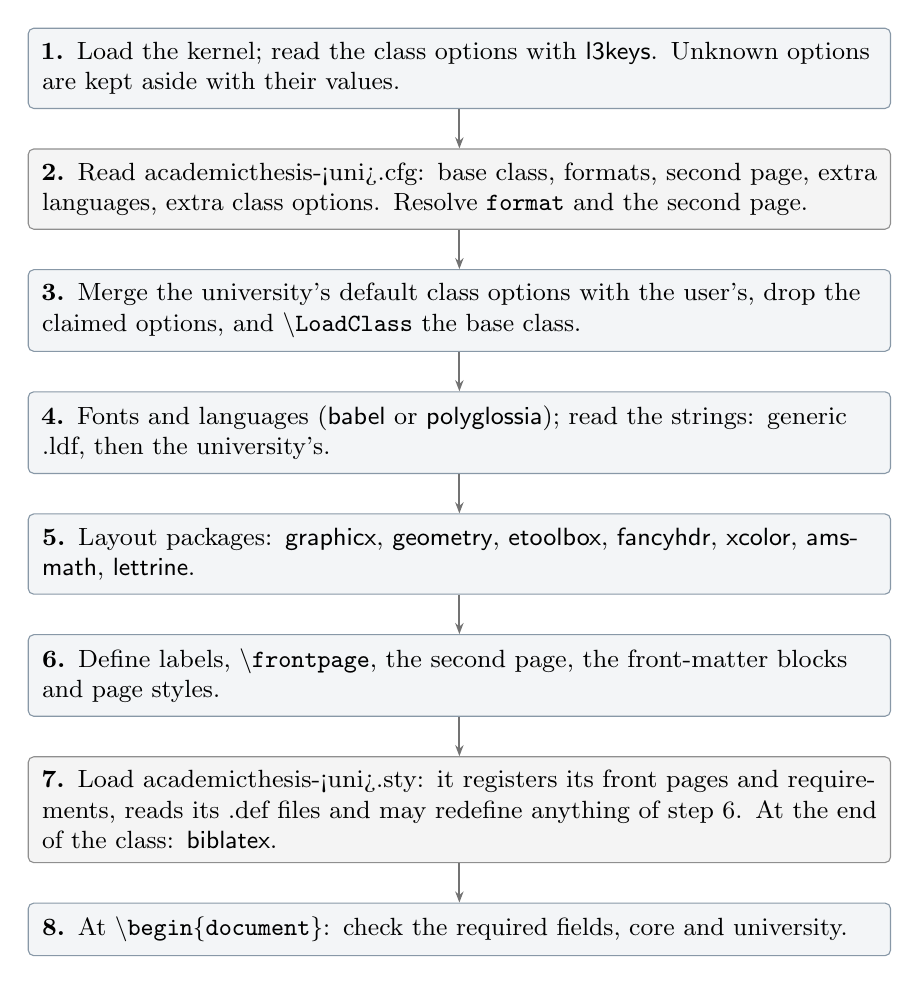
\begin{tikzpicture}[node distance=5mm,
    stepbox/.style={draw=docaccent!70, fill=docaccent!6, rounded corners=2pt,
      text width=10.6cm, align=left, font=\small, inner sep=5pt},
    unibox/.style={stepbox, draw=docgrey!80, fill=docgrey!8},
    arr/.style={-{Stealth[length=4pt]}, draw=docgrey, thick}]
  \node[stepbox] (s1) {\textbf{1.} Load the kernel; read the class options with \pkg{l3keys}. Unknown options are kept aside with their values.};
  \node[unibox, below=of s1] (s2) {\textbf{2.} Read \file{academicthesis-<uni>.cfg}: base class, formats, second page, extra languages, extra class options. Resolve \opt{format} and the second page.};
  \node[stepbox, below=of s2] (s3) {\textbf{3.} Merge the university's default class options with the user's, drop the claimed options, and \cs{LoadClass} the base class.};
  \node[stepbox, below=of s3] (s4) {\textbf{4.} Fonts and languages (\pkg{babel} or \pkg{polyglossia}); read the strings: generic \file{.ldf}, then the university's.};
  \node[stepbox, below=of s4] (s5) {\textbf{5.} Layout packages: \pkg{graphicx}, \pkg{geometry}, \pkg{etoolbox}, \pkg{fancyhdr}, \pkg{xcolor}, \pkg{amsmath}, \pkg{lettrine}.};
  \node[stepbox, below=of s5] (s6) {\textbf{6.} Define labels, \cs{frontpage}, the second page, the front-matter blocks and page styles.};
  \node[unibox, below=of s6] (s7) {\textbf{7.} Load \file{academicthesis-<uni>.sty}: it registers its front pages and requirements, reads its \file{.def} files and may redefine anything of step~6. At the end of the class: \pkg{biblatex}.};
  \node[stepbox, below=of s7] (s8) {\textbf{8.} At \cs{begin}\opt{\{document\}}: check the required fields, core and university.};
  \foreach \a/\b in {s1/s2,s2/s3,s3/s4,s4/s5,s5/s6,s6/s7,s7/s8} \draw[arr] (\a) -- (\b);
\end{tikzpicture}
\end{center}

Grey steps are where the university's own files run. Two consequences
matter when writing a university package:

\begin{itemize}
  \item The \file{.cfg} runs before \cs{LoadClass}: it may only use the
    early-configuration commands (Section~\ref{sec:cfg}) and \pkg{expl3}
    logic, not packages or document commands.
  \item The \file{.sty} runs \emph{after} the core has defined its
    labels, blocks and page styles (step~6), so a university redefines
    any of them directly, in its \file{.sty} or \file{.def}:
\begin{lstlisting}
\RenewDocumentCommand\thesiskeywords{mm}{...}
\fancypagestyle{Thesis}{...}
\end{lstlisting}
\end{itemize}

\section{The early configuration file}
\label{sec:cfg}

\file{academicthesis-<uni>.cfg} is read with \pkg{expl3} syntax on (spaces
are ignored; write \verb|~| for a space). Its commands concern only the
active university, so they take no university argument.

\begin{longtable}{@{}L{5.8cm} L{8.6cm}@{}}
\toprule
\textbf{Command} & \textbf{Meaning} \\
\midrule
\endhead
\cs{DeclareThesisBaseClass}\newline\opt{\{<class>\}\{<options>\}} & Base class (\pkg{book}, \pkg{article}, \dots) and its default options. A default is dropped when the user chose another option of the same group: \opt{11pt} beats a default \opt{12pt}, \opt{oneside} beats \opt{twoside}. Default: \pkg{book} with no options. \\
\cs{DeclareThesisFormats}\newline\opt{\{<list>\}\{<default>\}} & The values accepted by \opt{format=}. Resolved at once, so the rest of the file can branch on \cs{g\_\_academicthesis\_format\_tl}. A university that declares none rejects \opt{format=}. \\
\cs{DeclareThesisSecondPage}\newline\opt{\{true|false\}} & Default for the second page (examination commission and copyright). The user can override it with \opt{secondpage} / \opt{no-secondpage}. Default: \opt{true}. \\
\cs{DeclareThesisOtherLanguages}\newline\opt{\{<list>\}} & Languages always loaded with \pkg{babel}, besides the main one. \\
\cs{DeclareThesisClassOption}\newline\opt{\{<name>\}\{<default>\}} & Claims a \cs{documentclass} option for the university; it is no longer passed to the base class. \opt{name} alone means \opt{true}. Read it with \cs{academicthesis\_class\_option:n}\opt{\{<name>\}} or, in normal syntax, \cs{thesisclassoption}\opt{\{<name>\}}. \\
\cs{DeclareThesisCoreRequirements}\newline\opt{\{true|false\}} & Whether the core checks its own required fields (title, candidate, academic year, degree, supervisors). The university's requirements are checked either way. Default: \opt{true}. \\
\bottomrule
\end{longtable}

\section{Thesis data}

\subsection{The store}

All data given with \cs{thesissetup} goes into one global property list.
\cs{thesissetup} is a thin \pkg{l3keys} front-end: each key writes one
entry.

\begin{tabularx}{\textwidth}{@{}L{6.2cm} Y@{}}
\toprule
\textbf{\pkg{expl3} (in \file{.sty}/\file{.cfg})} & \textbf{Effect} \\
\midrule
\cs{academicthesis\_meta\_set:nn}\newline\opt{\{key\}\{value\}} & Store a value. \\
\cs{academicthesis\_meta\_get:n}\newline\opt{\{key\}} & The value (expandable; empty when missing). \\
\cs{academicthesis\_meta\_if\_empty:nTF} & Test for an empty or missing value (also \opt{p}, \opt{T}, \opt{F}). \\
\cs{academicthesis\_list\_set:nn}, \cs{\_set\_csv:nn}, \cs{\_add:nn} & Set a list to one item, to comma-separated items, or append one. \\
\cs{academicthesis\_list\_count:n}, \cs{academicthesis\_list\_if\_empty:nTF} & Number of items; emptiness test. \\
\bottomrule
\end{tabularx}

\begin{tabularx}{\textwidth}{@{}L{6.2cm} Y@{}}
\toprule
\textbf{Normal syntax (in \file{.def})} & \textbf{Effect} \\
\midrule
\cs{thesismeta}\newline\opt{\{key\}} & The value (expandable). \\
\cs{IfThesisMetaEmptyTF}\newline\opt{\{key\}\{empty\}\{not empty\}} & Branch on a value. \\
\cs{academicthesislist}\newline\opt{[sep]\{list\}} & Typeset a list; default separator \verb|\\|. \\
\cs{thesislistcount}\newline\opt{\{list\}}, \cs{IfThesisListEmptyTF} & Count items; branch on emptiness. \\
\cs{IfThesisDegreeTF}\newline\opt{\{bachelor|master|phd\}\{yes\}\{no\}} & Branch on the degree. \\
\cs{thesisclassoption}\newline\opt{\{name\}} & Value of a claimed class option. \\
\bottomrule
\end{tabularx}

The standard keys are \opt{title}, \opt{subtitle}, \opt{candidate},
\opt{idnumber}, \opt{degree}, \opt{chair}, \opt{department}, \opt{major},
\opt{phdtitle}, \opt{cycle}, \opt{academicyear}, \opt{copyyear},
\opt{examdate}, \opt{authoremail}, \opt{website}, \opt{dedication},
\opt{abstract}, \opt{keywords}, \opt{coordinator} and \opt{gender}, plus the
lists \opt{supervisors}, \opt{cosupervisors}, \opt{examiners} and
\opt{tutors} (each with a singular key that sets one item without
splitting at commas). A university may store keys of its own with
\cs{academicthesis\_meta\_set:nn}; the core never reads them.

\subsection{Validation}

At \cs{begin}\opt{\{document\}} the core checks its own fields (unless
switched off in the \file{.cfg}) and then every entry registered with

\begin{lstlisting}
\DeclareThesisRequirement{<uni>}{<boolean>}{<key>}{<example>}
\end{lstlisting}

whose university is the active one and whose \pkg{expl3} boolean is true:
\cs{c\_true\_bool} (always), \cs{g\_\_academicthesis\_bachelor\_bool},
\cs{\_master\_bool} or \cs{\_phd\_bool}. A missing field raises the error
\emph{Missing required thesis metadata: `<key>'}, whose help text shows
\opt{<example>}.

\section{Registries}

\begin{tabularx}{\textwidth}{@{}L{6.2cm} Y@{}}
\toprule
\textbf{Command} & \textbf{Meaning} \\
\midrule
\cs{DeclareThesisFrontPage}\newline\opt{\{<uni>\}\{<degree>\}\{<cs>\}} & \cs{frontpage} looks up \opt{<uni>.<degree>} and runs \opt{<cs>}; if nothing is registered, it raises \emph{No front page registered}. The command typesets its own page(s). \\
\cs{DeclareThesisRequirement}\newline\opt{\{<uni>\}\{<bool>\}\{<key>\}\{<ex>\}} & A required field (above). \\
\cs{DeclareThesisBibDefaults}\newline\opt{\{<uni>\}\{<options>\}} & \pkg{biblatex} options used when the user gives no \opt{biblatex-options}. \\
\bottomrule
\end{tabularx}

\section{Strings and languages}

Every printed word comes from a string store, one per language, filled by
\cs{ProvideThesisString}\opt{\{<key>\}\{<text>\}}. For each language the
kernel reads \file{academicthesis-<lang>.ldf} and then, if it exists,
\file{academicthesis-<uni>-<lang>.ldf}. A university file reuses the core
keys to change the wording (for instance \opt{SupervisorLabel}) and may add
keys of its own.

\cs{thesisstring}\opt{\{<key>\}} prints a string in the language currently
selected for strings: the main language, or the one a block switched to
with \opt{language=}. It falls back to the main language, then to the key
name, so a missing translation never stops compilation.

The labels \cs{authorlabel}, \cs{supervisorlabel} and \cs{cosupervisorlabel}
choose the singular or plural string from the length of the list, and the
female form of the candidate label from \opt{gender}.

\section{Front matter, second page, page styles}

\begin{itemize}
  \item \cs{frontpage} dispatches to the registered front page, then
    prints the second page if it is on.
  \item \env{abstractthesis}, \env{originality}, \env{acknowledgements}
    and \cs{dedication} all go through one option parser (\opt{language},
    \opt{title}, \opt{keywords}). Headings use \cs{thesisfrontchapter},
    which writes \cs{chapter*} or \cs{section*} depending on whether the
    base class has chapters, and adds the table-of-contents entry.
  \item Universities can restyle without touching the parser:
    \cs{thesiskeywords}\opt{\{<label>\}\{<keywords>\}} prints the keywords;
    \cs{thesisacknowledgementsbegin}\opt{\{<heading>\}} and
    \cs{thesisacknowledgementsend} frame the acknowledgements.
  \item The core defines the page styles \opt{Thesis}, \opt{acknowledgments}
    and \opt{plain}; \cs{frontmatter} switches to \opt{plain} and
    \cs{mainmatter} to \opt{Thesis}. Under a base class without chapters,
    the core supplies light versions of \cs{frontmatter}, \cs{mainmatter}
    and \cs{backmatter}.
\end{itemize}

\section{Two rules for writing layout code}
\label{sec:catcodes}

\paragraph{Typeset in normal syntax.} Under \cs{ExplSyntaxOn} spaces are
ignored and blank lines do not end paragraphs, which silently breaks any
text. University packages therefore keep their \pkg{expl3} code in the
\file{.sty} and put pages in \file{.def} files read with the document
catcodes:

\begin{lstlisting}
% kernel function: document catcodes, no group (definitions survive)
\academicthesis_input_layout:n { academicthesis-myuni-frontpage.def }
\end{lstlisting}

\paragraph{Never load a package from a \texttt{.def} file.} When a package
loaded from there ends, \LaTeX{} restores the syntax of the class that is
loading everything, \pkg{expl3}, and every space that follows is lost. The
\file{.sty} loads the packages before reading the \file{.def}.

\section{Search path in the repository}
\label{sec:searchpath}

Inside the repository the files sit in sub-folders, which \TeX{} does not
search. Two mechanisms make them visible without any path in the code:

\begin{itemize}
  \item \textbf{latexmk}: the root \file{latexmkrc} adds \file{core//},
    \file{languages//} and \file{universities//} to \opt{TEXINPUTS} (the
    trailing \opt{//} also searches sub-folders).
  \item \textbf{Any editor}: \file{showcases/academicthesis-repo-paths.tex},
    input before \cs{documentclass}, extends \LaTeX's \cs{input@path} with
    the folders. \cs{input@path} does not search sub-folders, so it lists
    each university folder; a new university needs a line there.
\end{itemize}

\section{Messages}

All messages use the \pkg{expl3} message module \opt{academicthesis}, so
they read \emph{Class academicthesis Error} and carry a help text.

\begin{tabularx}{\textwidth}{@{}l Y@{}}
\toprule
\textbf{Name} & \textbf{When} \\
\midrule
\opt{missing-metadata} & A required field is empty. \\
\opt{missing-frontpage} & No front page registered for the university and degree. \\
\opt{unknown-university} & No \file{academicthesis-<uni>.sty} found. \\
\opt{missing-config} & The \file{.sty} exists but the \file{.cfg} does not. \\
\opt{unknown-format}, \opt{no-formats} & A \opt{format} the university does not declare, or any \opt{format} at a university with none. \\
\opt{missing-language} & No \file{.ldf} for the chosen language (falls back to English). \\
\opt{bibliography-fallback} & \pkg{biblatex} unavailable (warning). \\
\bottomrule
\end{tabularx}

A university defines its own messages in the same module with
\cs{msg\_new:nnnn}\opt{\{academicthesis\}\{<uni>-<name>\}\{...\}\{...\}}.

\section{Adding a university, in short}

\begin{enumerate}
  \item Create \file{universities/<uni>/} with
    \file{academicthesis-<uni>.cfg} (at least \cs{DeclareThesisBaseClass}).
  \item Write \file{academicthesis-<uni>.sty}: \cs{RequirePackage}
    \opt{\{academicthesis-kernel\}}, setup keys, packages, requirements,
    then read the \file{.def} files.
  \item In each \file{.def}, define the front page and register it with
    \cs{DeclareThesisFrontPage} for each degree offered.
  \item Add \file{academicthesis-<uni>-<lang>.ldf} files for its wording.
  \item Add its folder to \file{showcases/academicthesis-repo-paths.tex}
    and a showcase.
\end{enumerate}

Nothing in \file{core/}, \file{languages/} or another university changes.


% ======================================================================
\chapter{The PoliMi package}
\label{ch:unidev}

\begin{notebox}{Origin of the layout code}
The layout files re-implement Politecnico di Milano's official templates
(Scuola 3I, October 2021; PhD template by J.~Stevens and L.~Fossati).
Measurements, colours and heading styles are taken from those templates;
when changing them, compare with the originals.
\end{notebox}

\section{Files}

\begin{tabularx}{\textwidth}{@{}l Y@{}}
\toprule
\textbf{File} & \textbf{Role} \\
\midrule
\file{academicthesis-polimi.cfg} & Formats, base class per format, the \opt{phd} rule, no second page, English and Italian always loaded. \\
\file{academicthesis-polimi.sty} & \cs{polimithesissetup}, requirements per format, packages per format, reading the format's \file{.def}. \\
\file{academicthesis-polimi-classical.def} & Classical layout. \\
\file{academicthesis-polimi-article.def} & Article layout. \\
\file{academicthesis-polimi-summary.def} & Executive Summary layout. \\
\file{academicthesis-polimi-phd.def} & Doctoral dissertation layout. \\
\file{academicthesis-polimi-english.ldf}, \file{-italian.ldf} & PoliMi wording of core strings, and PoliMi-only strings. \\
\file{logopolimi3i.pdf}, \file{raggierapolimi.pdf}, \file{logopolimiseal.png} & Scuola 3I logo, background, PhD seal (converted from the templates). \\
\file{academicthesis-polimi-doc.tex} & The package's own short manual. \\
\bottomrule
\end{tabularx}

\section{The early configuration}

The \file{.cfg} is where the four formats become four base classes:

\begin{lstlisting}
% the phd degree defaults to the phd format
\bool_if:NT \g__academicthesis_phd_bool
  { \tl_if_empty:NT \g__academicthesis_format_tl
      { \tl_gset:Nn \g__academicthesis_format_tl { phd } } }
\DeclareThesisFormats { classical , article , summary , phd } { classical }
% format=phd needs the phd degree (error polimi-phd-needs-phd)

\str_case:VnF \g__academicthesis_format_tl
  {
    { classical } { \DeclareThesisBaseClass { book }    { 12pt , twoside , a4paper } }
    { article }   { \DeclareThesisBaseClass { article } { 11pt , a4paper } }
    { summary }   { \DeclareThesisBaseClass { article } { 11pt , a4paper , twocolumn } }
    { phd }       { \DeclareThesisBaseClass { book }    { 10pt , twoside , openright } }
  }
  { ... }
\DeclareThesisSecondPage { false }
\DeclareThesisOtherLanguages { english , italian }
\end{lstlisting}

Because \cs{DeclareThesisFormats} resolves the format at once, the rest of
the file can branch on it. The core then merges these defaults with the
user's options and loads the class.

\section{The package}

\paragraph{1. Options.} \cs{polimithesissetup} sets the key family
\opt{academicthesis-polimi/layout}: \opt{logo-file} (default chosen by
format: \opt{logopolimiseal} for \opt{phd}, \opt{logopolimi3i} otherwise),
\opt{watermark} (the switch \cs{ifpolimi@watermark}) and \opt{paper} (runs
\cs{polimi@paper@17x24} or \cs{polimi@paper@a4}, defined by the PhD
layout). \cs{polimi@logofile} gives the logo to the layout files.

\paragraph{2. Requirements.} On top of the core's (title, candidate,
degree, supervisors, academic year): \opt{idnumber} for \opt{classical}
and \opt{article}; \opt{department}, \opt{phdtitle} and \opt{cycle} for
\opt{phd}; \opt{abstract} for \opt{article}.

\paragraph{3. Packages per format,} loaded from the \file{.sty} (never from
a \file{.def}):

\begin{tabularx}{\textwidth}{@{}l Y@{}}
\toprule
\textbf{Format} & \textbf{Packages} \\
\midrule
\opt{classical} & \pkg{titlesec}, \pkg{caption}, \pkg{setspace}, \pkg{eso-pic}, \pkg{transparent}, \pkg{amsthm} \\
\opt{article} & \pkg{titlesec}, \pkg{caption}, \pkg{eso-pic}, \pkg{transparent}, \pkg{amsthm} \\
\opt{summary} & \pkg{titlesec}, \pkg{caption}, \pkg{eso-pic}, \pkg{transparent}, \pkg{amsthm} \\
\opt{phd} & Times / Helvetica / Courier (TeX Gyre with Lua\LaTeX), \pkg{caption}, \pkg{amsthm}, \pkg{fncychap} (Sonny), \pkg{titlesec} (calcwidth), \pkg{tocloft} (titles) \\
\bottomrule
\end{tabularx}

The blue boxes of \opt{article} and \opt{summary} (keywords, page header)
are a \cs{colorbox} with the template's padding and spacing, so
\pkg{tcolorbox} (and TikZ) is not loaded. For \opt{phd}, the obsolete
\pkg{times} package is replaced by the same fonts set directly
(pdf\LaTeX) or their TeX Gyre clones (Lua\LaTeX, Xe\LaTeX).

\paragraph{4. The layout.} Finally the \file{.sty} reads, with the
document catcodes, \file{academicthesis-polimi-common.def} (classical,
article, summary: colour, theorem style, section headings, watermark
macro, blue box, thesis-type line), then
\file{academicthesis-polimi-<format>.def}.

\section{The layout files}

All four follow the same plan, in numbered sections:

\begin{enumerate}
  \item \textbf{Page, paragraphs}: \cs{geometry}, spacing (the colour
    \opt{bluepoli} and the drop-cap colour are in the common file).
  \item \textbf{Captions and theorems}: \env{theorem} and
    \env{proposition} with the common \opt{polimi} style, numbered within
    chapters or sections (PhD: \env{defn}), labels from \cs{thesisstring}.
  \item \textbf{Headings} with \pkg{titlesec}. The classical format also
    redefines \cs{chapter} so that starred chapters reach the table of
    contents and the running header.
  \item \textbf{Watermark}: the raggiera placed with \pkg{eso-pic}
    (\cs{AddToShipoutPicture*}) on the cover, page~1 or blank pages, through
    the common \cs{polimi@watermark}\opt{\{x\}\{y\}\{width\}}; the
    classical format redefines \cs{cleardoublepage} for that.
  \item \textbf{Front page}: \cs{polimi@frontpage}, registered for the
    degrees of that format:
\begin{lstlisting}
\DeclareThesisFrontPage{polimi}{bachelor}{\polimi@frontpage}
\DeclareThesisFrontPage{polimi}{master}{\polimi@frontpage}
% academicthesis-polimi-phd.def:
\DeclareThesisFrontPage{polimi}{phd}{\polimi@frontpage}
\end{lstlisting}
  \item \textbf{Core pieces redefined} (directly: the core has defined
    them before loading the package): the page styles
    \opt{Thesis} and \opt{plain}, \cs{thesisfrontchapter},
    \cs{thesiskeywords} (the blue box in \opt{article} and \opt{summary})
    and the acknowledgements frame.
\end{enumerate}

Metadata is read with \cs{thesismeta}, \cs{IfThesisMetaEmptyTF},
\cs{IfThesisListEmptyTF} and \cs{IfThesisDegreeTF}; labels with
\cs{thesisstring}.

\section{Strings}

\file{academicthesis-polimi-<lang>.ldf} changes the wording of core keys
(\opt{CandidateLabel} = Author, \opt{IDNumber} = Student ID,
\opt{SupervisorLabel} = Advisor, \opt{CoSupervisorLabel} = Co-advisor) and
adds PoliMi keys: \opt{BachelorThesisIn}, \opt{MasterThesisIn},
\opt{CoverAbstractLabel}, \opt{ExecutiveSummaryOfThesis},
\opt{ExecutiveSummaryHeader}, \opt{DoctoralDissertationOf},
\opt{PhDSupervisorLabel(s)}, \opt{TutorLabel(s)}, \opt{CoordinatorLabel},
\opt{DefinitionLabel}, \opt{TheoremLabel}, \opt{PropositionLabel}.

\section{Common changes}

\begin{tabularx}{\textwidth}{@{}L{5cm} Y@{}}
\toprule
\textbf{To change\dots} & \textbf{Edit\dots} \\
\midrule
a cover or first-page block & section~5 (PhD: 4) of that format's \file{.def}. \\
headings, captions, theorems & sections 2--3 of that format's \file{.def}. \\
running headers, keywords, acknowledgements & the last section of that format's \file{.def}. \\
colour, section headings, blue box, watermark & \file{academicthesis-polimi-common.def}. \\
a label's wording & \file{academicthesis-polimi-<lang>.ldf}. \\
required fields & section~2 of the \file{.sty}. \\
default class options of a format & the \file{.cfg}. \\
\bottomrule
\end{tabularx}

\paragraph{Adding a format.} Add it to \cs{DeclareThesisFormats} and to
the base-class switch in the \file{.cfg}, list its packages in the
\file{.sty}, and write \file{academicthesis-polimi-<format>.def} with its
front page registered by \cs{DeclareThesisFrontPage}.

% ======================================================================
\chapter*{Licence and credits}
\addcontentsline{toc}{chapter}{Licence and credits}

\pkg{academicthesis} is released under the \LaTeX{} Project Public Licence
(LPPL) 1.3c or later; copyright 2025--2026 Luca Salvatore.

The layouts of the PoliMi package are based on the official \LaTeX{}
templates of Politecnico di Milano: the Scuola 3I thesis templates
(classical format, article format, Executive Summary; revision of October
2021) and the PoliMi doctoral dissertation template by J.~Stevens and
L.~Fossati. Their design, and the Politecnico di Milano name, logos, seal
and graphic elements, belong to Politecnico di Milano and to the
templates' authors. \pkg{academicthesis} is not published by Politecnico
di Milano: before submitting, check the current rules of your school or
doctoral programme.

\end{document}
